\chapter{Technologies}\label{sec:chap:2}

For the last 40 years society has been living the third industrial revolution, better known as the digital age. Telecommunications and technological innovations are transforming the way people live and work, one way these innovations have impacted society is by allowing users to connect cheaper and quicker internationally, making it easier to share ideas than ever before. 
The ever-growing number of bots assisting humans has allowed companies to automate more and more, relieving people from the most boring of jobs, this has resulted in a higher demand for higher educated workers specially in computer science and other engineering areas. 
As you can see in the graph below, people are becoming more interested in these areas. This helps further develop these technologies as the more people interested, the more ideas are shared and more progress is done.\\

\begin{center}
	\begin{figure}[h!]
		\centering
		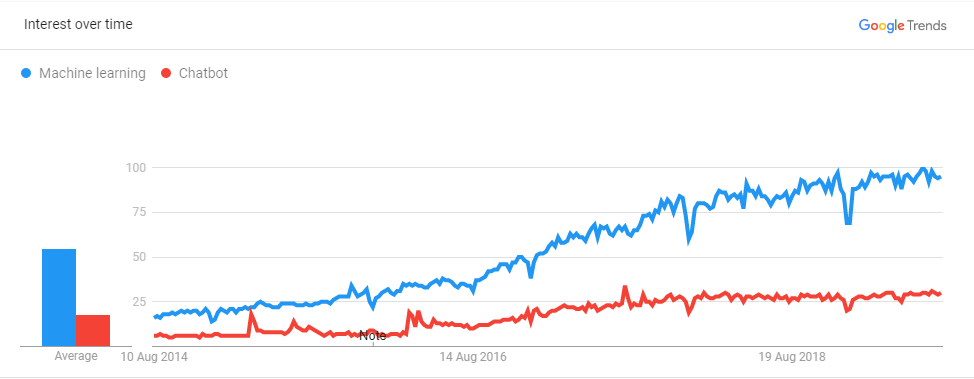
\includegraphics[scale=0.6]{./images/3-mach-chat-trend}
		\caption{Global Trends for Machine Learning and Chatbots}
		\label{global-trends-mach-chat}
	\end{figure}
\end{center}

In this chapter the background for the technologies that were used in the project will be explained. \\

\section{Artificial Intelligence}\label{sec:chap3_ai}
As Andrew Ng, a professor from Stanford said, AI is the new electricity, in a certain way the same as electricity changed many industries, AI is set to revolutionize the world. But before explaining further, let’s explain what Artificial Intelligence is. Based on Encyclopaedia Britannica’s definition, AI is the ability for digital computers of performing tasks commonly associated with intelligent beings.  There are two main ways of classifying AI:\\
\begin{itemize}
	\item {\textbf{Type 1:}
		\begin{itemize}
			\item {\textbf{Strong AI:} This is an AI that thinks just like a human. Currently there are no examples of this happening, but its development has accelerated innovations in AI.}
			\item {\textbf{Weak AI:} Build machines that do things like humans but without an understanding of how the human brain works. It is where a machine only is able of doing one task.}
		\end{itemize}
	Companies normally develop a fusion between these two types where machines have a partial understanding of how humans work to do tasks.\\
	}
	\item {\textbf{Type 2:}
		\begin{itemize}
			\item {\textbf{Reactive Machines:} One of the more basic types of Artificial Intelligence. It can’t use past information to do future actions. It focuses more on rules than actual knowledge.}
			\item {\textbf{Limited Memory:} In this case the AI can use past information to do future actions. This design for AI has been integrated in autonomous vehicles, where the car stores information of what occurs in its surroundings. This functionality is used also in chatbots to maintain a contextual idea of the conversation as the machine stores relevant information to make it more human-like.}
			\item {\textbf{Theory of Mind:} This is where a machine can understand and interpret human emotions, beliefs, thoughts, etc. By understanding what makes us human it can be able to socially interact with them. This would be the next level for chatbots, now the machine can extract a person’s emotion by the words and tone spoken with and respond differently based on that, but still has a way to go to understanding humans.}
			\item {\textbf{Self-awareness:} Still in the science fiction stage where a machine is conscious, intelligent and aware, basically a human being. If human kind reaches this point in AI, it would be a huge milestone for the field but will also raise many questions.}
		\end{itemize}
	}
\end{itemize}

Many people confuse Artificial Intelligence with machine learning, but this is wrong, machine learning is a part of AI, many other areas encompass the whole of AI. To visualize this easier the image before shows you how 	this areas are divided.\cite{ai}\\

\begin{center}
	\begin{figure}[h!]
		\centering
		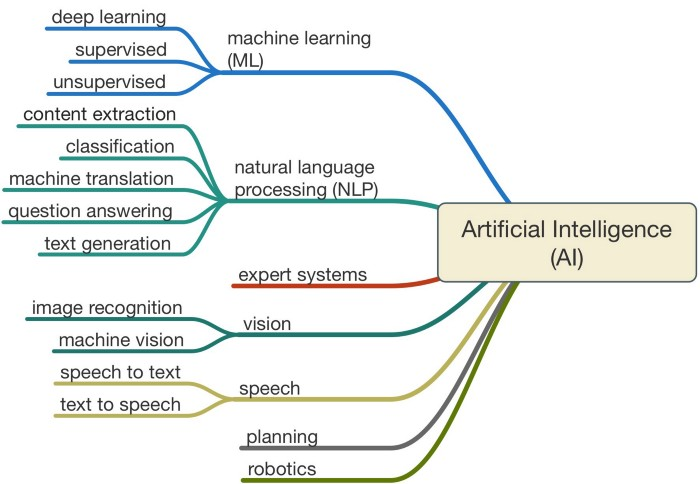
\includegraphics[scale=0.5]{./images/3-ai-areas}
		\caption{Areas in Artificial Intelligence}
		\label{ai-areas}
	\end{figure}
\end{center}

For this project the main areas that were used from AI are Machine Learning and Natural Language Processing. For a final product, speech would be an upgrade to the project to make it able to interact through voice with the user.\\

\begin{itemize}
	\item {\textbf{Machine Learning:} For this project we use supervised training where the bot has conversations with a trainer that tells what the bot should do based on what the user says.}
	\item {\textbf{Natural Language Processing:} Even though many of the tools provided are integrated in Rasa, several tools where used for the bot to work in the initial iteration of the chatbot and still requires tweaking with Rasa.\\
		
		\begin{itemize}
			\item {\textbf{Content Extraction:} This is where valuable information is extracted from what the user says, this can be what can of training they are seeking, at what time they want to be reminded to take their measurements or when the user was born. This is done by using regular expressions or by using lists with synonyms, depending of what type of info is extracted.}
			\item {\textbf{Classification:} Depending on what the user says, the bot must understand what his intentions are, this is done by training the bot with training phrases that reflect what does the user want and associating it with an intention, after training a model, the bot is able to distinguish between different intentions. Before training the bot, human phrases must be translated to something the machine can understand.}
		\end{itemize}
			}
\end{itemize}

\section{Chatbots}\label{sec:chap3_ai}
A chatbot is a software based on AI that simulates a human conversation with a user. This is done through messaging applications such as Telegram, Facebook, websites or company’s messaging software.\\

Chatbots have been slowly but steadily been incorporated into people’s lives, from basic robo-calls to natural speaking bots used in customer service. Virtual assistants such as Google or Alexa, that are constantly getting feature updates making bigger the number of things they can do, such as ordering pizza or getting a booking for a restaurant. These improvements have to do with many of the technologies involved, that have improved greatly. We will explain below the different components in a chatbot and how its architecture has evolved.\\

\subsection{Messaging Platform}\label{sec:chap3_cha_mes_pla}
The messaging app is where the user interacts with the chatbot. As mentioned previously there are several ways of communicating with the chat bot, it can be written or spoken. Depending on how the user talks with the chat bot there will be additional processing, because if the user uses spoken language it must be transcribed for the machine to understand.\\

\subsection{Natural Language Processor}\label{sec:chap3_cha_nlp}
The Natural Language Processor is the step where the bot does most of the work. When the message is received it goes through a series of conversions.\\

\begin{itemize}
	\item {\textbf{Speech to Text:} This is needed only when the message sent from the user is in voice format, such as the virtual assistants solutions provided by Google or Amazon, although this can also be included in applications where voice messages functionality is available.}
	\item {\textbf{Language Detection:} This is a way of building a multilingual chatbot without the need of building different models for every language. The issue is how to get the translation, there is a well-known API from google that provides this functionality for a price. A way to reduce costs can be to have a cache store the most frequent translations.}
	\item {\textbf{Tokenizing:} In this step what the bot does is separate the phrases in independent words, it is also important for the bot to understand what each word is, if it is a noun, verb, adjective or an adverb. Also, it must discard all redundant words that don’t provide any additional information.}
	\item {\textbf{Stemming:} This consists in simplifying the words in the phrase in order to have a much simpler vocabulary for the bot to understand, this is done by eliminating verb conjugations or keeping the stem of the word. In the image below there is a more in detail example of what stemming is.\cite{cha-stem}}
	
	\begin{center}
		\begin{figure}[h!]
			\centering
			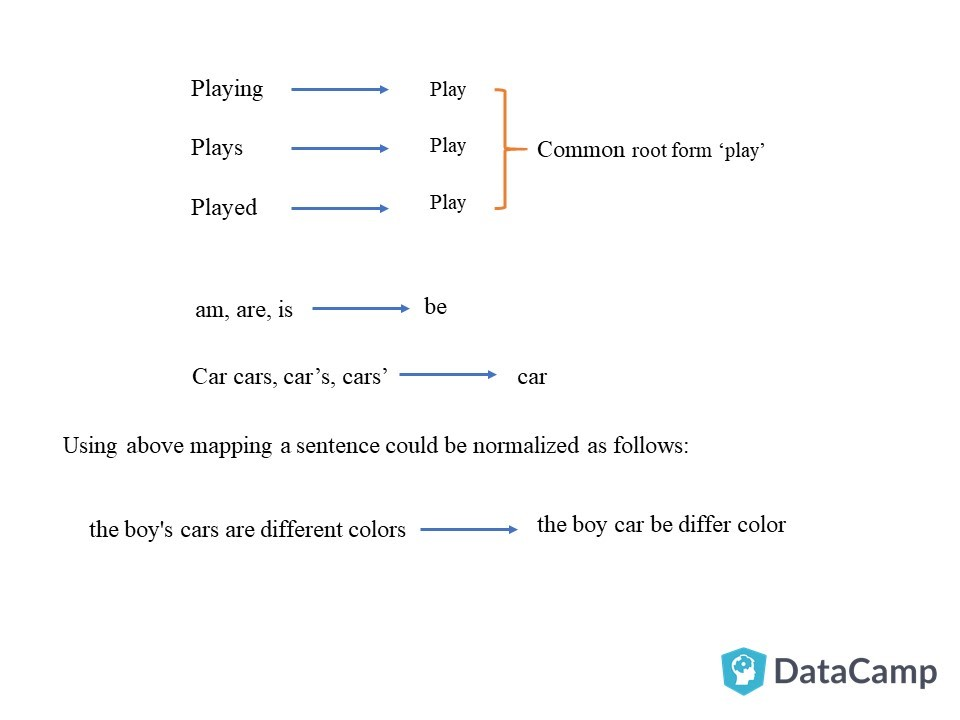
\includegraphics[scale=0.7]{./images/3-chatbot-stemming}
			\caption{Stemming Examples}
			\label{cha_stem}
		\end{figure}
	\end{center}

	\item {\textbf{Word to number:} The bot in at this point translates the tokenized and stemmed words into numbers the bot can understand, this is done in two steps.\\
			\begin{itemize}
				\item {\textbf{Word Identifier:} In this step what the bot does is convert each word with a numerical identifier. In this way, for example all the hello’s will be number 1. This helps the bot in the next step.}
				\item {\textbf{Term Frequency:} Here what the bot does is check the frequency of certain words in the training data. This will be used to help classify as some words are more frequent in some intents more than in others.}
			\end{itemize}	
		}
	\item {\textbf{Intent detection:} Based on the frequency words show up on the user’s message the bot can predict what the user’s intention is.}
	\item {\textbf{Entity Extraction:} Once the intent is predicted the next step is extracting the information that is relevant to that intent, in case of setting a reminder for example it is important for the bot to understand at what time does the user wants to be reminded.\\
	This can be done in several ways:\\ 
			\begin{itemize}
				\item {Regular expressions to extract information that comes in certain formats.}
				\item {Lists for finite proper names, like cities or countries.}
				\item {By adding many examples of the data that you want the bot to extract.}
				\item {Filling the missing information with user relevant info extracted in previous occasions.}
				\item {Asking the user for the missing information.}
			\end{itemize}
		}
	\item {\textbf{Response:} After extracting all the relevant information from the user’s message create a response that answers the user’s request and perform whichever action needs to be performed.}
\end{itemize}

\subsection{Profiler}\label{sec:chap3_cha_pro}
The profiler is an extension of the chatbot that allows it to become much more intuitive and natural with the conversations. What the profiler does is gather information from the user through their previous conversations, then uses that info to give context to the user’s requests or fills out missing information based on the user’s preferences.\\

For example, in this project when the user asks to be reminded to take his measurements at 8 am, the bot will extract that information for future occasions. If after that interaction the user asks to be reminded the next day the bot will automatically use the hour extracted from the previously without asking the user for that information.\\

\begin{center}
	\begin{figure}[h!]
		\centering
		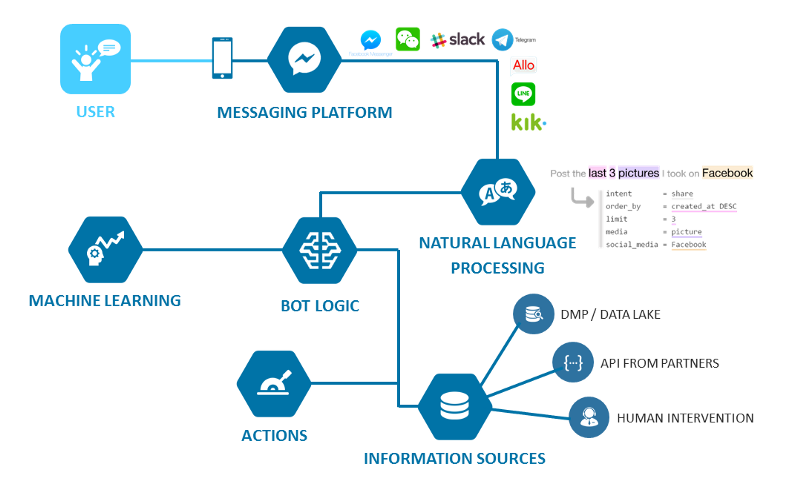
\includegraphics[scale=0.6]{./images/3-cha-struct}
		\caption{Chatbot Architecture}
		\label{cha_struct}
	\end{figure}
\end{center}

\subsection{Chatbot Platforms}\label{sec:chap3_plat}

There are many platforms to build chatbots, with their own features. Below there is a table of the difference between several solutions. In this section we will talk about some of them and what differences each have.\\


\begin{table}[h!]
	\centering
	\resizebox{\linewidth}{!}{
		\begin{tabular}{|c|c|c|c|c|} 
			\hline
			\rowcolor[rgb]{0.753,0.753,0.753} Bot Name                                                               & Features                                                                                                                                                                                                                                           & Technical Details                                                                                                                                                                           & License                                                                                                                                  & Channel                                                        \\ 
			\hline
			\begin{tabular}[c]{@{}c@{}}IBM Watson \\Conversation Service \end{tabular}                               & \begin{tabular}[c]{@{}c@{}}Has three main components: \\Intents, \\Entities, \\Dialog\\ \\ Analysis, to detect what\\~messages confuse the bot \end{tabular}                                                                                       & \begin{tabular}[c]{@{}c@{}}Built on a neural network \\(one billion Wikipedia words). \end{tabular}                                                                                         & \begin{tabular}[c]{@{}c@{}}Free, priced \\per message,\\ \\ Contact required \\for enterprise \end{tabular}                              & \begin{tabular}[c]{@{}c@{}}Voice\\ Image\\ Text \end{tabular}  \\ 
			\hline
			Wit.ai                                                                                                   & \begin{tabular}[c]{@{}c@{}}Home automation\\ \\ Wearables\\ \\ Hardware \end{tabular}                                                                                                                                                              & \begin{tabular}[c]{@{}c@{}}Allows to use:\\ \\ Entities\\ Intents\\ Context\\ Actions \end{tabular}                                                                                         & Free                                                                                                                                     & \begin{tabular}[c]{@{}c@{}}Voice\\ Text \end{tabular}          \\ 
			\hline
			Rasa                                                                                                     & \begin{tabular}[c]{@{}c@{}}Interactive Learning\\ \\ Stories \end{tabular}                                                                                                                                                                         & \begin{tabular}[c]{@{}c@{}}Modular Pipeline to \\design what best fits for you \end{tabular}                                                                                                & Open Source                                                                                                                              & Text                                                           \\ 
			\hline
			Dialogflow                                                                                               & \begin{tabular}[c]{@{}c@{}}Intuitive Platform\\ \\ Pretrained packages \\from Google\\ \\ Chit Chat built in \end{tabular}                                                                                                                         & \begin{tabular}[c]{@{}c@{}}Neural Network\\ \\ Black box \end{tabular}                                                                                                                      & \begin{tabular}[c]{@{}c@{}}Free\\ Enterprise \end{tabular}                                                                               & \begin{tabular}[c]{@{}c@{}}Voice\\ Text \end{tabular}          \\ 
			\hline
			\begin{tabular}[c]{@{}c@{}}Microsoft Language \\Understanding\\~Intelligent Service (LUIS) \end{tabular} & \begin{tabular}[c]{@{}c@{}}All LUIS applications are \\centered around a \\domain-specific topic or\\ content related.\\ \\ Active learning.\\ \\ You can use pre-existing, \\world-class, pre-built \\models from Bing and Cortana. \end{tabular} & \begin{tabular}[c]{@{}c@{}}LUIS offers a set of \\programmatic REST APIs \\that can be used by\\ developers to automate \\the application creation process. \end{tabular}                   & \begin{tabular}[c]{@{}c@{}}Free\\{[}10.000 Transactions]\\Paid\\{[}1,50\$1.000 transactions]\\{[}4,50\$ 1.000transactions]~\end{tabular} & \begin{tabular}[c]{@{}c@{}}Voice\\ Text \end{tabular}          \\ 
			\hline
			Pandorabots                                                                                              & \begin{tabular}[c]{@{}c@{}}AIML (Artificial Intelligence \\Markup Language) \\ \\ Includes A.L.I.C.E. \end{tabular}                                                                                                                                & \begin{tabular}[c]{@{}c@{}}The Pandorabots API allows \\you to integrate our bot \\hosting service and\\ \\ natural language \\processing engine into \\your own application. \end{tabular} & \begin{tabular}[c]{@{}c@{}}Free\\Developer [19\$/month]\\Pro [199\$/month]\\~Enterprise [Sales]~ ~~\end{tabular}                         & Text                                                           \\
			\hline
		\end{tabular}
	
	}
\label{cha_diff}
\caption{Differences between different chatbot solutions}
\end{table}
 

\subsubsection{DialogFlow}\label{sec:chap3_dialog}

Dialogflow is Google’s solution for chatbots. It is a framework that uses Google’s ML expertise and offers the user an attractive and intuitive web design. It let’s the user create a chatbot that can interpret text and voice.\\
The difference between Dialogflow and Rasa is that the latter gives the developer more freedom when creating the brains of the chatbot, this can be good or bad. For it to be good, it requires lots of data and knowledge in the field. The advantage Dialogflow has over Rasa for less technical people, is that everything done with the NLU Engine is mostly done already, that leaves the developers with teaching the bot how they want it to perform.\cite{dialogflow}\\

The core functionality is composed of several components:\\
\begin{itemize}
	\item {\textbf{Events:} These are actions that are taken based on the intent, they depend on what the developer wants to do with the chatbot.}
	\item {\textbf{Entities:} Like many chatbot frameworks, entities are the information that the bot must extract from a phrase.}
	\item {\textbf{Context:} In Dialogflow there are two types of context, input context and output context.\\
			\begin{itemize}
				\item {Input Context is a required condition that must be set in in order to trigger the intent. An example would be after setting one alarm, the user asks to set another one. If it wasn’t for the previous context the chatbot would have a hard time understanding it.}
				\item {Output Context is what the intent sets after being triggered for the chatbot to understand what has happened before.}
			\end{itemize}
			}
	\item {\textbf{Intents:} The action the user wants to perform. In Dialogflow all intents are managed with an interface where the developers add the intent it wants predicted and chooses what context, event or entities they want extracted.}
\end{itemize}


\subsubsection{Rasa}\label{sec:chap3_rasa}

\begin{center}
	\begin{figure}[h!]
		\centering
		
\includegraphics[scale=0.3]{./images/3-rasa-log}
		\caption{Rasa Logo}
		\label{rasa_logo}
	\end{figure}
\end{center}

Rasa is an open source platform that offers several tools to build a contextual chatbot, in other words, a bot that can maintain a history of what the user says.\\
The reason for choosing this platform to build the chatbot is that it is open source, free and has the features required, which are:

\begin{itemize}
	\item Option to choose a customized pipeline, modifying it to improve the bot’s accuracy.
	\item Tools to build the chatbot with pretrained entities or custom ones.
	\item Built in system to maintain the context in a conversation.
	\item Tool that allows the user to teach the chatbot through conversation.
	\item Ability to connect to messaging applications.
	\item Tool to create custom actions to certain intents.
	\item Ability of using reminders to send messages to user’s at certain times.
\end{itemize}
	
The problem with using this solution is that you are limited by what is available and what functionality you can add, another limitation compared to Dialogflow is that the only support you can get comes from the users, this isn’t to helpful when you need urgent assistance as you have to wait for a user to answer. Even though there is documentation to assist developers when creating the chatbot the documentation lacks many details on how many things are done and. what the best practices are. This depending on how much Rasa grows, might improve over time.\\
There are two main components in rasa, NLU and CORE, each can work independently if the client’s requirements needs it or they can work together. We will explain how each component works.\cite{rasa}\\

\textbf{\underline{NLU}}\\

Rasa NLU is an open-source natural language processing tool for intent classification and entity extraction in chatbots.  From the user’s message it translates it to a JSON data object with the intent predicted and the entities extracted from the message.\\

For example, from the following message it returns the data structure shown below. With intent, search\_restaurant and entities cuisine and location.

\begin{lstlisting}
message = "I am looking for a Mexican restaurant in the center of town"

response = {
	"intent": "search_restaurant",
	"entities": {
		"cuisine" : "Mexican",
		"location" : "center"
	}
}

\end{lstlisting}

The benefits of Rasa NLU when comparing it to Dialogflow is that you can choose your own pipeline. A pipeline is a series of components that together create the Natural Language Processor. There are components for intent classification, components for entity extraction and preprocessing. Each component sends it’s output to the next output to extract all relevant information from the message, so even though there are several components there will only be one output as shown below.

\begin{center}
	\begin{figure}[h!]
		\centering
		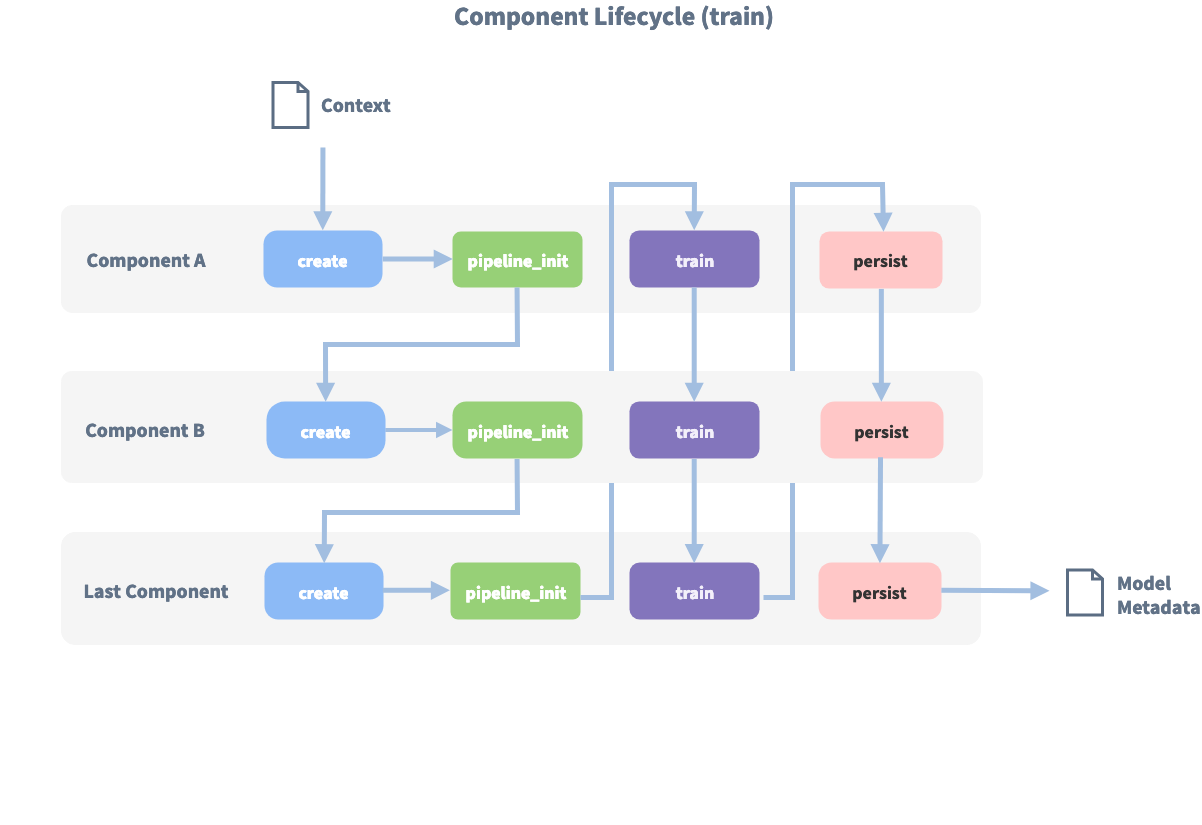
\includegraphics[scale=0.4]{./images/3-rasa-pipe}
		\caption{Rasa Pipeline}
		\label{rasa_pipe}
	\end{figure}
\end{center}

There are two main pipelines already built and ready to use with Rasa.
\begin{itemize}
	\item {\textbf{pretrained\_embeddings\_spacy:} This pipeline comes with the word vectors, relation between words in a given context, already trained which makes this a very good pipeline for a short training list, less than 1000.}
	\item {\textbf{supervised\_embeddings:} This is different than the pipeline above in the way that it isn’t pretrained which means that it will create the word vectors based on the dataset available, this is only recommended when a larger dataset is available as it requires a lot of data to interpret it correctly
		}
\end{itemize}
There are custom pipelines, where you create it based on what components the developer wants to have. Adding components for sentiment analysis or different components to classify intents.\\

\textbf{\underline{CORE}}\\

Rasa Core is a dialogue engine used for building virtual assistants, it has several parts that makes treating conversations easier.
\begin{itemize}
	\item {\textbf{Stories:} This is the main component of the core, it is a representation of the conversation flow, with intents and actions. This teaches the bot to know what actions to perform depending on what the user says. Below there is an example of how a story looks like.
	\begin{lstlisting}
	## story_07715946    <!-- name of the story - just for debugging -->
	* greet
	- action_ask_howcanhelp
	* inform{"location": "rome", "price": "cheap"}  <!-- user utterance, in format intent{entities} -->
	- action_on_it
	- action_ask_cuisine
	* inform{"cuisine": "spanish"}
	- action_ask_numpeople        <!-- action that the bot should execute -->
	* inform{"people": "six"}
	- action_ack_dosearch
	
	\end{lstlisting}
	}
	\item {\textbf{Slots:} This is the chatbots memory, it is a way of controlling the context of the conversation as the bot can remember what information the user has said previously and guide the user and/or perform some action based on the information.}
	\item {\textbf{Forms:} A very useful tool that allows the bot to extract information from the user, the difference with setting the slots is that with forms it is quicker to setup for when the bot needs several elements of information as it checks if the user has said any relevant information in the message. For the case, “I want to book a Chinese restaurant for 8” the form will extract “Chinese” and “8” and will only ask the user for the missing information for the booking.}
	\item {\textbf{Actions:} This is something performed in the background that may be search something in a DB, call an API or setting slots.}
	\item {\textbf{Interactive learning:} When adding more complexity to the chatbot this becomes a very useful way of training it as the developer maintains a conversation with the bot and teaches it what to do depending on the conversation flow.}
\end{itemize}

\section{Databases}\label{sec:chap3_db}

Databases are key parts of software development, used basically in every application out there. What they provide is the functionality of storing data relevant to the service the application provides. In the case of a bank, databases may store information on a person’s bank account or credit rating. The structuring and managements of databases has become a major area in the development of software. Where its design is key for scalability, security and maintenance.

\subsection{Evolution}\label{sec:chap3_db_evo}

Before databases where used, all data relevant to a company had to be stored in paper, when the company is small or the data it has to store is minimal it isn’t a big problem, but rarely this is the case and companies have to store large amount of data on paper where the security and management of these files becomes a tedious one, as to search for something specific a person has to look over lot’s of data, another issue is that if a fire broke out all the history of an entity would be wiped out. Databases provided a solution to this problem by digitalizing the company’s data. The earliest database systems where the hierarchical and network models.

\begin{itemize}
	\item {\textbf{Hierarchical model:} It organizes data in a tree like structure, this model was created in the 1960’s. It is an easy to understand model as it simulates an enterprise structure. Even though the model was created in the 1960’s it is still in use in some applications to this date. You can see this model in use in a computers file system. The problem with this model is that every time a record wanted to be accessed the whole tree had to be traversed.

	\begin{center}
		\begin{figure}[h!]
			\centering
			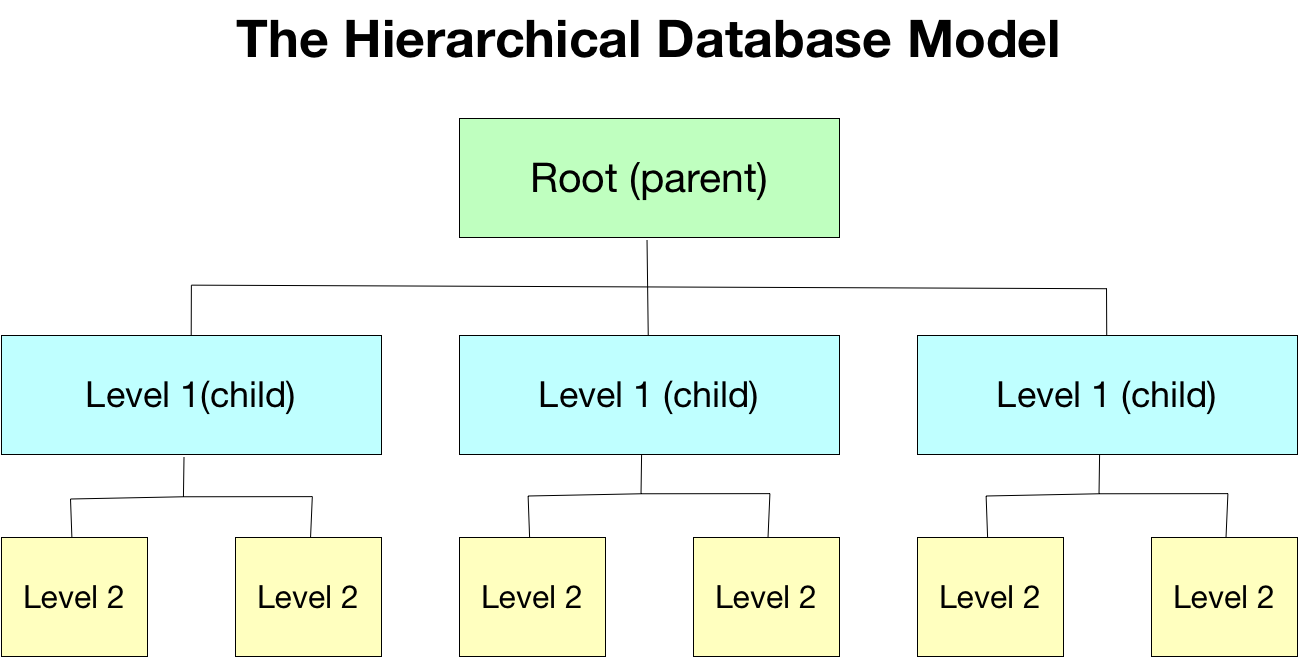
\includegraphics[scale=0.22]{./images/3-hierarchical-model}
			\caption{Hierarchical Model}
			\label{hier_model}
		\end{figure}
	\end{center}
	}
	
	\item {\textbf{Network model:} In 1969 a new model was announced that solved some of the limitations from the hierarchical model, which is that each node can be related with another node from the tree even if it isn’t from the same branch. Even if this model offered improvements it wasn’t massively used as IBM continued developing its products with the hierarchical model.
	\begin{center}
		\begin{figure}[h!]
			\centering
			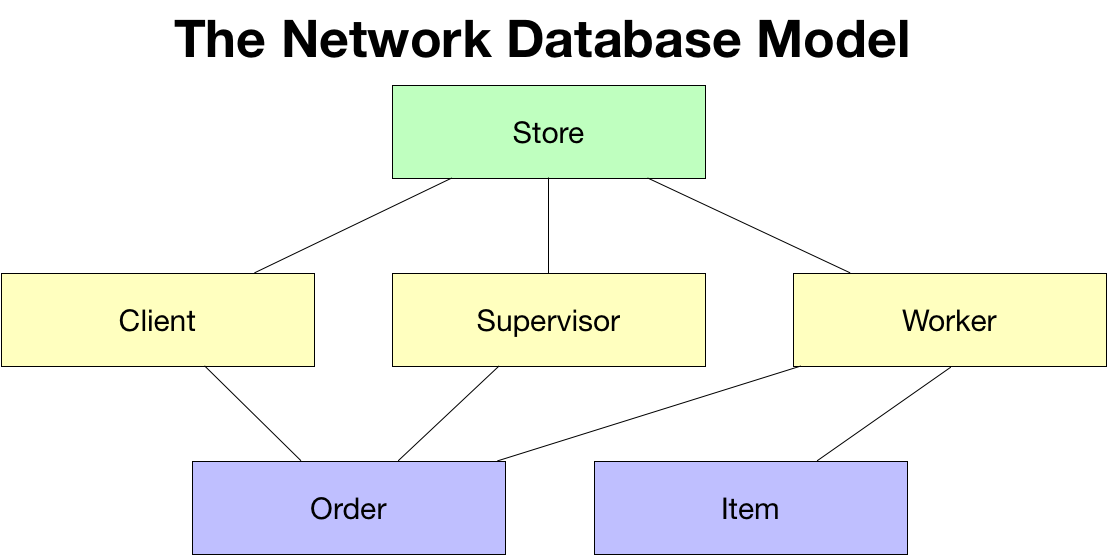
\includegraphics[scale=0.25]{./images/3-network-model}
			\caption{Network Model}
			\label{net_model}
		\end{figure}
	\end{center}
	}
	\item {\textbf{Relational model:} This model was easier to understand, and the programming interface was better. The problem was that when this model came to light, at the same time as the network model, it couldn’t be used due to limiting computer power, this in the 1980s was overcome by breakthroughs in the computing industry.\\
	This model differs from the other two models as it uses tables to store data, this data can be related with other tables making it a very attractive solution and making it easier to maintain.\\
	There are three ways of relating data in this model:
	\begin{itemize}
		\item {One-to-One}
		\item {One-to-Many}
		\item {Many-to-Many}
	\end{itemize}
	\begin{center}
		\begin{figure}[h!]
			\centering
			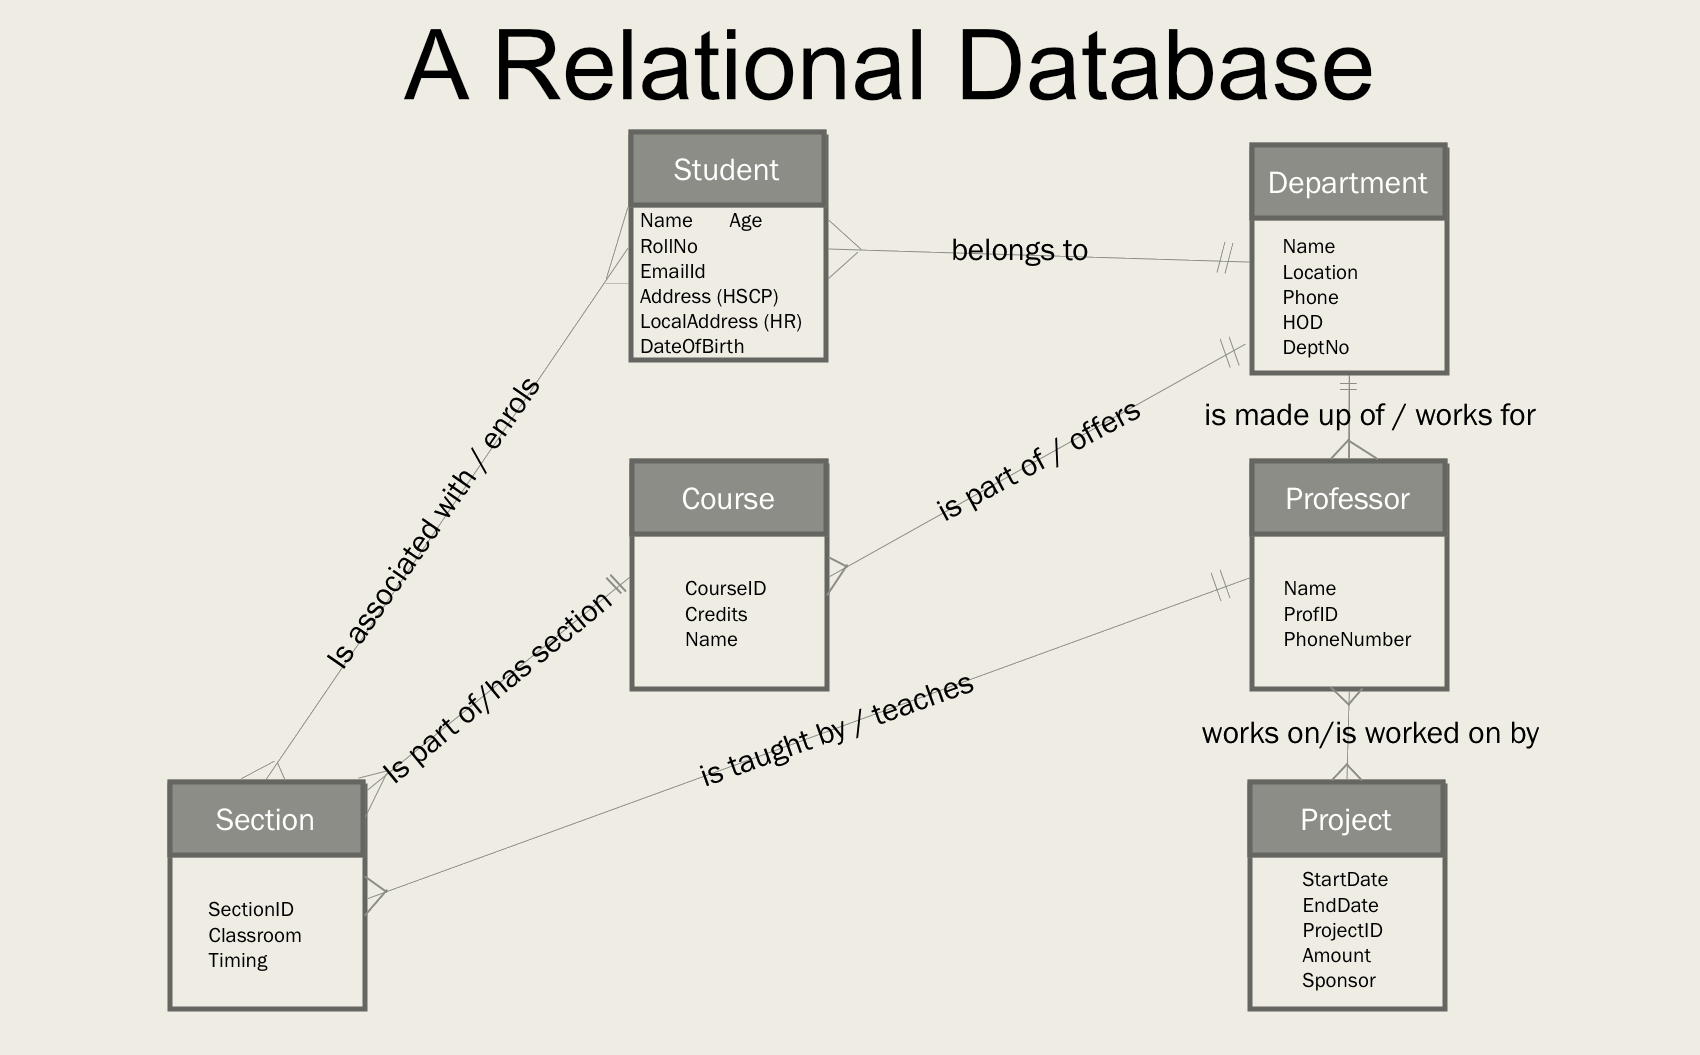
\includegraphics[scale=0.20]{./images/3-relational-model}
			\caption{Relational Model}
			\label{rel_model}
		\end{figure}
	\end{center}
	The language this model used is called Structured Query Language (SQL), there are several variations to this language depending on the application being used. Soon this became the standard and started being used in enterprise environments. In the mid-1990s a revolution in the development came about and new open sourced software with no cost for the developer started getting traction and with it the open source project of MySQL, which first version was developed by a Swedish company. The fact it was free, lowered the entry barrier for new developments.
	}
	\item {\textbf{NoSQL:} In 1998 a new term was created, NoSQL that categorized all databases that didn’t follow the same language as the most common relational databases. They came about with the internet boom, this was because a shift was coming around and more and more data was being ingested by the database. SQL databases have a harder time scaling up, with more demand in internet traffic and speed becoming the focus on the server-side, new ways of storing data had to be developed. It focuses more in simplicity and maintenance as it is easier to add new fields to existing data. 
	\begin{center}
		\begin{figure}[h!]
			\centering
			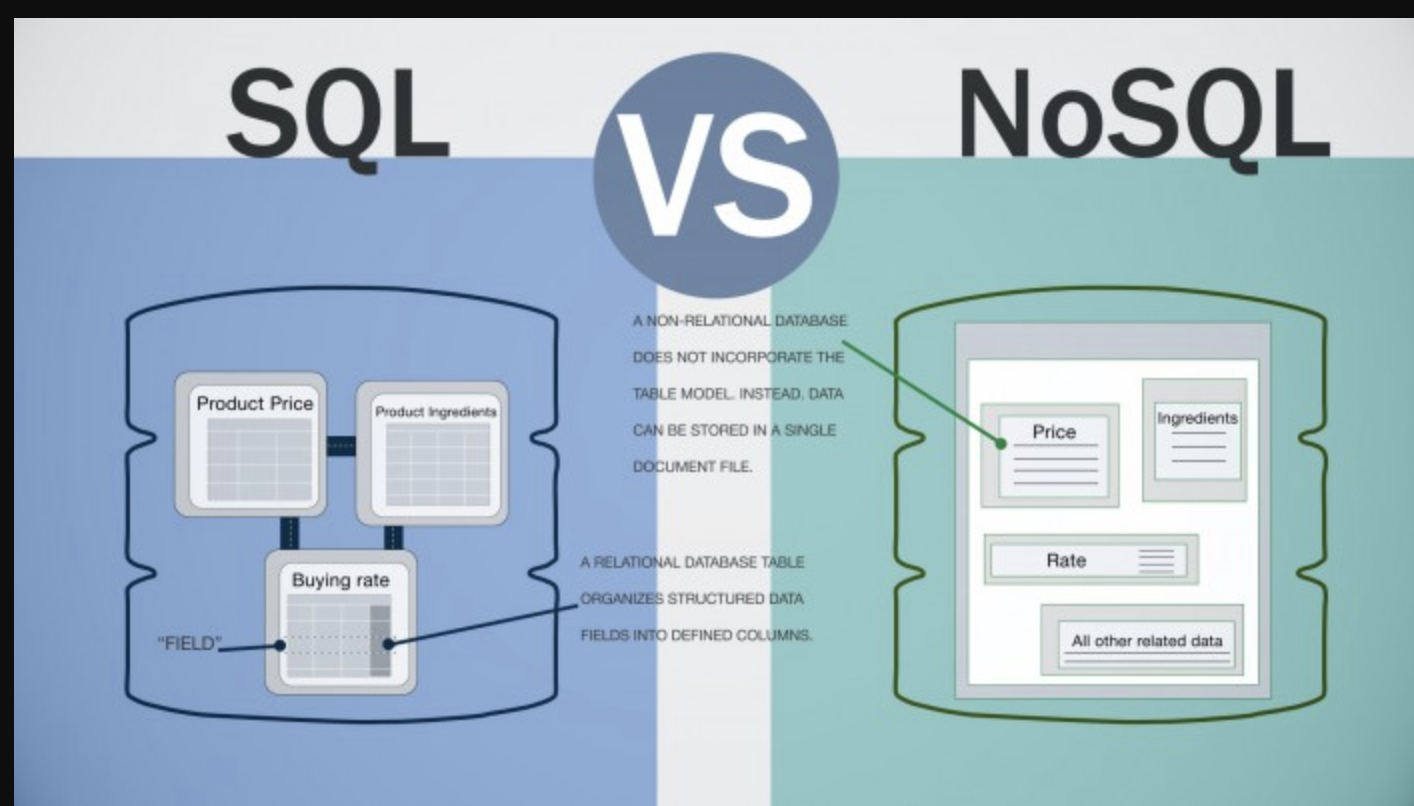
\includegraphics[scale=0.25]{./images/3-nosql}
			\caption{SQL vs NoSQL}
			\label{nosql}
		\end{figure}
	\end{center}
	Big Data has played a major role in the last few years, with storage prices in decline and the affordability of storing large amounts of data, has allowed scientists to analyze data to extract relevant information. This data is not only structured, created using applications or employees, it is data that can be extracted from unstructured sources. This can be comments from people on a product or if a media campaign is causing any impact. This information is highly valuable and that is why companies are so invested in it.\cite{db-hist}
	}
\end{itemize}
\clearpage
\subsection{Solutions}\label{sec:chap3_db_sol}
In this section we will expand on some of the solutions available for SQL and NoSQL databases.

\subsubsection{NoSQL}\label{sec:chap3_db_nosql}
This are some of the solutions for NoSQL databases, there is also on-premises or cloud databases that can be used.

\begin{table}[h!]
	\centering
	\resizebox{\linewidth}{!}{
		\begin{tabular}{|l|l|}
			\hline
			\rowcolor[HTML]{C0C0C0} 
			Name            & Description                                                                                                                                                                                                         \\ \hline
			\rowcolor[HTML]{96FFFB} 
			\multicolumn{2}{|c|}{\cellcolor[HTML]{96FFFB}On-Premise}                                                                                                                                                                              \\ \hline
			MongoDB         & \begin{tabular}[c]{@{}l@{}}Most\\ popular database, uses json-like documents to store data, which makes it much\\ more expressive.\end{tabular}                                                                     \\ \hline
			Redis           & \begin{tabular}[c]{@{}l@{}}An open-source, distributed database that uses key-value to store\\   data which makes it very fast to extract data.\end{tabular}                                                        \\ \hline
			Cassandra       & \begin{tabular}[c]{@{}l@{}}Open-source database created by Facebook with the focus on scalability\\   and high availability.\end{tabular}                                                                           \\ \hline
			\rowcolor[HTML]{96FFFB} 
			\multicolumn{2}{|c|}{\cellcolor[HTML]{96FFFB}Cloud}                                                                                                                                                                                   \\ \hline
			\rowcolor[HTML]{9B9B9B} 
			\multicolumn{2}{|c|}{\cellcolor[HTML]{9B9B9B}AWS}                                                                                                                                                                                     \\ \hline
			DynamoDB        & \begin{tabular}[c]{@{}l@{}}Key-value and document database that offers high scalability with database\\   management automated.\end{tabular}                                                                        \\ \hline
			DocumentDB      & \begin{tabular}[c]{@{}l@{}}Compatible with MongoDB, offers high performance, it has the compute\\   and storage elements separated to have more flexibility on scaling the\\   database.\end{tabular}               \\ \hline
			\rowcolor[HTML]{9B9B9B} 
			\multicolumn{2}{|c|}{\cellcolor[HTML]{9B9B9B}Microsoft Azure}                                                                                                                                                                         \\ \hline
			CosmosDB        & \begin{tabular}[c]{@{}l@{}}Azure solution that allows the use of different NoSQL models with the\\   functionality of scaling dynamically across the globe.\end{tabular}                                            \\ \hline
			\rowcolor[HTML]{9B9B9B} 
			\multicolumn{2}{|c|}{\cellcolor[HTML]{9B9B9B}Google Cloud}                                                                                                                                                                            \\ \hline
			Bigtable        & \begin{tabular}[c]{@{}l@{}}A very low latency solution that like other solutions focuses mainly\\   on scalability and availability. Allows easy integration with big data tools.\end{tabular}                      \\ \hline
			Cloud Firestore & \begin{tabular}[c]{@{}l@{}}Offers high availability with data replication, more expensive solution\\   than Bigtable, the main difference is that it offers better functionality for\\   transactions.\end{tabular} \\ \hline
	\end{tabular}}
	\label{nosql_tab}
	\caption{NoSQL Solutions}
\end{table}



\clearpage
\subsubsection{SQL}\label{sec:chap3_db_sql}
There are solutions both for on premises and cloud, some use the same language while others offer their own language.

\begin{table}[h!]
	\centering
	\resizebox{\linewidth}{!}{
		\begin{tabular}{|l|l|}
			\hline
			\rowcolor[HTML]{C0C0C0} 
			Name               & Description                                                                                                                                                                                           \\ \hline
			\rowcolor[HTML]{96FFFB} 
			\multicolumn{2}{|c|}{\cellcolor[HTML]{96FFFB}On-Premise}                                                                                                                                                                   \\ \hline
			MySQL              & \begin{tabular}[c]{@{}l@{}}The\\ most popular open-source SQL database.\end{tabular}                                                                                                                  \\ \hline
			PostgreSQL         & \begin{tabular}[c]{@{}l@{}}Focused more on the enterprise side, it offers higher extensibility than\\   MySQL.\end{tabular}                                                                           \\ \hline
			Oracle             & \begin{tabular}[c]{@{}l@{}}Offers the full service, but comes at a high price, used more by big enterprises\\   that can’t risk security mismanagement.\end{tabular}                                  \\ \hline
			\rowcolor[HTML]{96FFFB} 
			\multicolumn{2}{|c|}{\cellcolor[HTML]{96FFFB}Cloud}                                                                                                                                                                        \\ \hline
			\rowcolor[HTML]{9B9B9B} 
			\multicolumn{2}{|c|}{\cellcolor[HTML]{9B9B9B}AWS}                                                                                                                                                                          \\ \hline
			RDS                & \begin{tabular}[c]{@{}l@{}}Amazons own relational database solution, it offers a platform available\\   with different database engines such as MySQL, PostgreSQL, Oracle and many more.\end{tabular} \\ \hline
			Aurora             & A database engine that focuses on a higher throughput and scalability.                                                                                                                                \\ \hline
			\rowcolor[HTML]{9B9B9B} 
			\multicolumn{2}{|c|}{\cellcolor[HTML]{9B9B9B}Microsoft Azure}                                                                                                                                                              \\ \hline
			Azure SQL Database & Their own proprietary solution for a cloud database.                                                                                                                                                  \\ \hline
			Azure Database     & A solution compatible with existing SQL engines such as MySQL or PostgreSQL.                                                                                                                          \\ \hline
			\rowcolor[HTML]{9B9B9B} 
			\multicolumn{2}{|c|}{\cellcolor[HTML]{9B9B9B}Google Cloud}                                                                                                                                                                 \\ \hline
			Cloud SQL          & \begin{tabular}[c]{@{}l@{}}A google platform to use with database engines such as PostgreSQL or\\   MySQL.\end{tabular}                                                                               \\ \hline
			Cloud Spanner      & Solution that combines SQL elements with NoSQL.                                                                                                                                                       \\ \hline
	\end{tabular}}
	\label{sql_tab}
	\caption{SQL Solutions}
\end{table}


\section{Raspberry Pi}\label{sec:chap3_rasp}
A raspberry pi is a small single board computer with very low power consumption. Although limited in computing power its processor is still capable of running many programs and with recent models the hardware as gotten more powerful while maintaining its low price.\\

\begin{center}
	\begin{figure}[h!]
		\centering
		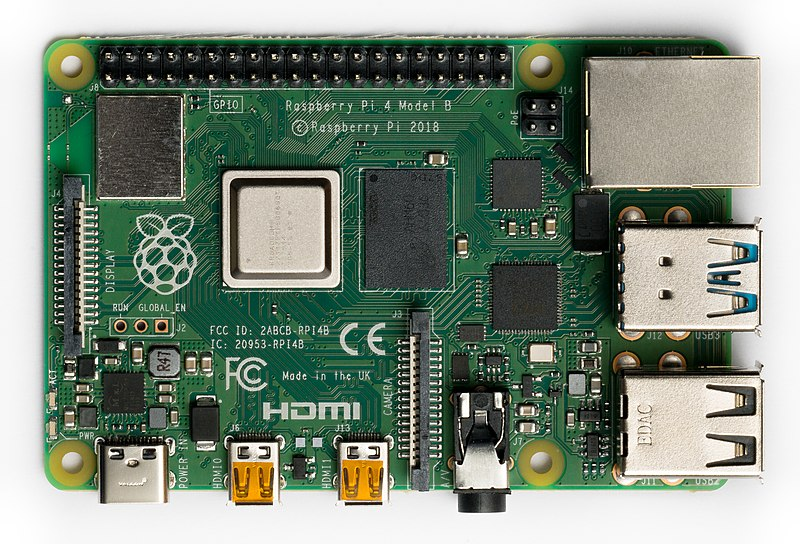
\includegraphics[scale=0.32]{./images/3-rasp-4}
		\caption{Raspberry Pi 4B}
		\label{rasp}
	\end{figure}
\end{center}

The Raspberry Pi has an ARM architecture processor which even though it benefits the pc on its low power requirements, it has compatibility issues with some software that is built for the x86 x64 processors.

The Raspberry Pi has many uses and as an affordable pc, here is a list of some examples to show the potential this device has, the limit to what you can do with a low powered computer are up to the developer’s imagination.

\begin{itemize}
	\item {\textbf{Media center:} You can configure the Raspberry Pi to act as a place to store or load films to watch on the users tv.}
	\item {\textbf{Retro gaming machine:} It can be used to remember old retro games by using the Raspberry Pi as an emulator for old games.}
	\item {\textbf{Game streaming:} Another option is using it as a device for games, streaming from the pc to the tv.}
	\item {\textbf{Security camera:} As it has an IO interface the developer can add modules like cameras and us it for surveillance to keep a house safe or check on the baby.}
	\item {\textbf{Home automation:} Having access to the local network the Raspberry Pi can be used as the brains of the house and use it to check data on the temperature, turn the heating on and plenty more.}
	\item {\textbf{Server:} The Raspberry Pi can also be used as a server, although limited in computing power it still has capability to be used for projects or as a development server.}
\end{itemize}

\subsection{Clusters}\label{sec:chap3_clusters}
A cluster is a set of computers that are tightly or loosely connected to work with each other, it acts like a single system, using the different computers to balance the load or for specific tasks.\\
For more intense projects these clusters may be required, the advantage the raspberry pi has is that its affordable price and small size factor the developer can build a powerful system with them. It can be used to balance the load on a web server. It can also be used as a mini supercomputer by supporting large amounts of cores and a large amount of RAM memory.

\section{Cloud Services}\label{sec:chap3_cloud}

Originally every company that wanted to manage their data and applications had to have a on-premises server to manage it, this required technical people having to be hired for the maintenance and upgrades the server required, when a company’s business model isn’t related to servers this becomes a burden. Another issue this causes is if not enough money is invested on this the availability of the server would be bad, and if it had to offer services in different countries latency becomes an issue.\\

Cloud computing offers a solution to these issues, a company can custom select what type of system they need to build their infrastructure, this can adapt to the companies needs in relation to processing power or storage space, this means that if a company focuses in the storage and transfer business they can build an infrastructure that focuses more on capacity, transfer speed and storage speed, compared to another company that works with artificial intelligence that may need a more powerful computer and less storage  space. This becomes available thanks to the improvements on virtualization.

\subsection{Virtualization}\label{sec:chap3_vir}

\begin{center}
	\begin{figure}[h!]
		\centering
		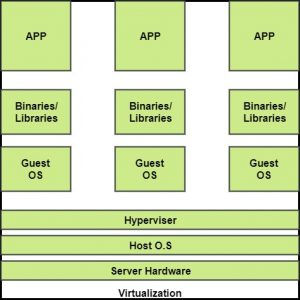
\includegraphics[scale=1]{./images/3-cloud-vir}
		\caption{Virtualization System}
		\label{cloud_vir}
	\end{figure}
\end{center}

Virtualization is a technique that separates the physical layer from the service level, this allows that a computer with certain resources have several virtual operating systems on top with different resources allocated. This offers many benefits in relation to cloud computing.

\begin{itemize}
	\item{Dynamic allocation of resources}
	\item{Lower costs of infrastructure}
	\item{Rapid scalability and remote access}
	\item{Multiple parallel OS}
	\item{Pay for time resources used}
\end{itemize}

There are different types of virtualization for different parts of the computer:

\begin{itemize}
	\item{\textbf{Storage virtualization:} This allows several servers storage as a single system, this virtualization allows it to be redundant as it offers tools for data replication and recovery, so if a server fails or a hard drive gets damaged the data remains intact.}
	\item{\textbf{Desktop virtualization:} This virtualization allows the user of the virtual system to access it remotely without knowing in what machine the OS is located.}
	\item{\textbf{Network virtualization:} The ability to create virtual networks to connect different elements in the data center allows different services to be able to communicate with each other.}
	\item{\textbf{Application virtualization:} With this type of virtualization different versions of a same application can coexist and allows an application to run without being installed in the traditional way or be supported by an OS.}
\end{itemize}

\subsection{Providers}\label{sec:chap3_prov}

\begin{itemize}
	\item{\textbf{AWS:} Amazon Web Services launched on 2006 and pioneered the business model for on-demand cloud computing, it has the highest market share of all the providers available. It offers a very large selection of products to choose from, making it better to create a well-defined architecture. AWS focuses more in the public cloud making enterprises with their own data center hard to interoperate with AWS.}
	\item{\textbf{Google Cloud:} The underdog in the competition between AWS and Microsoft Azure, it doesn’t have an enterprise focus which makes it harder to attract enterprise clients. It provides services with deep learning and machine learning which google cloud has leading technology.}
	\item{\textbf{Microsoft Azure:} A close competitor from Amazon Web Services, with years of experience and close relations with many enterprises Microsoft Azure offers what these clients want, that is to operate Azure functionality mixed with their own data center, allowing for a hybrid cloud.}
\end{itemize}

\section{Testing}\label{sec:chap3_test}

Testing is an essential part of software development which allows code to be bug free, even though it may seem tedious at the beginning in the long run it pays off and other developers will appreciate a built testing infrastructure.\\
There are several types of testing:\cite{testing}

\begin{itemize}
	\item {\textbf{Unit tests:} These are the lowest level of testing, where individual methods and functions are tested to verify that they are working correctly. Unit tests are easy to automate and are quite common in continuous integration, where in every new build it verifies that anything previous is working correctly.}
	\item {\textbf{Integration tests:} These tests are higher level where different modules or services work well with each other. The complication of running these tests is that it requires certain parts of the application to be running.}
	\item {\textbf{Functional tests:} Focusing more on the business requirements, these tests only are interested in the result not the middle steps between starting the action and the result. It differentiates from integration testing is that integration tests are only interested in checking if the system works and functional testing is more interested in verifying that the result is correct.}
	\item {\textbf{End-to-end tests:} End-to-end testing simulates user behavior to test if the flows of the application are working correctly. It is a very high level of testing and it is more complicated to automate due to needing interaction directly with the application, this interaction if automated needs to be maintained because any update on the interface of the application can render the test useless.}
	\item {\textbf{Performance testing:} This type of tests is very important to have when building big applications as it provides relevant information on how scalable the application is and if any significant latency or crashes are noticed.}
	\item {\textbf{Smoke testing:} Like functional tests but less expensive, just to verify the main systems are operational, if the deployment is functional then more expensive tests can be run.}
\end{itemize}

\subsection{Automation}\label{sec:chap3_auto}

Having a person run the tests above is possible but it would be very expensive, counter-productive and a very boring job as they must run every time a deployment or a new feature is added. To automate the tests programmatically the developer needs a testing framework that suits the application. These frameworks are dependent of the programming language used. Even though this automation allows to execute tests to verify the application the next step is to whenever the developer chooses to deploy the application, the tests run automatically before deploying, this is called continuous integration.